\newgeometry{left=1in, right=1in, top=1in, bottom=1.2in}

\chapter{Introduction}
\section{Project Overview}
Used car price prediction is a practical supervised learning problem that aims to estimate the selling price of a previously owned vehicle from its characteristics and market information. In this project, a regression-based workflow was developed and evaluated on a used-car dataset to understand which factors influence price and how accurately they can be used for prediction.

The dataset contains information about vehicle name, year of manufacture, selling price, kilometres driven, fuel type, seller type, transmission, and owner history. Because the target variable is continuous and the predictors include both numerical and categorical features, regression methods are well suited for this task.

\section{Objectives}
The main objectives of this study were to:
\begin{itemize}
  \item build a predictive model for used car price estimation;
  \item investigate how vehicle age, mileage, and categorical attributes affect selling price;
  \item compare simple and regularized regression approaches; and
  \item present the workflow and results in a structured technical report.
\end{itemize}

\chapter{Dataset and Methodology}
\section{Dataset Description}
The dataset used in this study was obtained from Kaggle and contains records for used cars with multiple attributes that are relevant to pricing. The target variable is the selling price, while the predictors describe the vehicle's condition and market context.

The dataset contains 4,340 records and no missing values. The numerical variables include the model year, selling price, and kilometres driven, while the categorical variables include fuel type, seller type, transmission, owner type, and the vehicle name itself. These features are useful because they capture both the intrinsic value of the car and the market signals that influence resale price.

\section{Experimental Setup}
The analysis followed a clear regression workflow:
\begin{enumerate}
  \item load and inspect the data;
  \item visualize the distributions of the main variables;
  \item explore relationships between price and the predictors;
  \item encode categorical features for modelling; and
  \item train and evaluate regression models using train-test and cross-validation procedures.
\end{enumerate}

The modelling study focused on baseline linear regression and regularized linear methods. These approaches were chosen because they provide interpretable baselines and a useful reference point for understanding whether the relationships in the data are approximately linear.

\chapter{Exploratory Data Analysis}
\section{Distribution of Variables}
A first look at the dataset shows that many vehicles are concentrated in the mid-2000s to late-2010s model years, while kilometres driven is strongly right-skewed. The selling price distribution is also skewed, with a small number of high-value vehicles sitting far above the majority of observations. This pattern is common in used-car markets, where premium vehicles and newer models command a substantially higher resale value.

\begin{figure}[H]
  \centering
  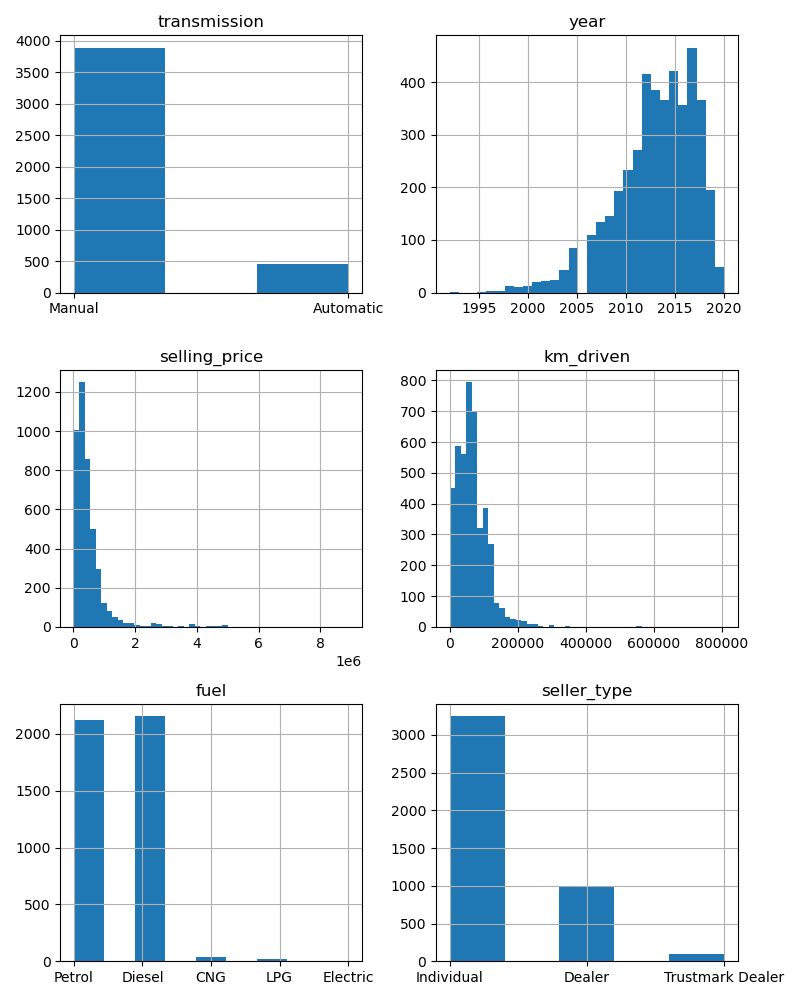
\includegraphics[width=0.95\textwidth]{../figures/variable_distributions.png}
  \caption{Distribution of the main vehicle attributes and the target variable.}
\end{figure}

The categorical variables also show clear market patterns. Petrol vehicles dominate the sample, manual transmission is more prevalent than automatic transmission, and individual sellers form the largest seller-type category. These distributions suggest that the dataset captures a broad but somewhat heterogeneous market segment.

\section{Relationship Between Price and Predictors}
The relationship between selling price and the main features was explored using scatter plots and category-wise comparisons. The plots indicate that newer vehicles tend to have higher selling prices, while vehicles with greater mileage are usually priced lower. This makes intuitive sense because age and usage are strong indicators of depreciation.

\begin{figure}[H]
  \centering
  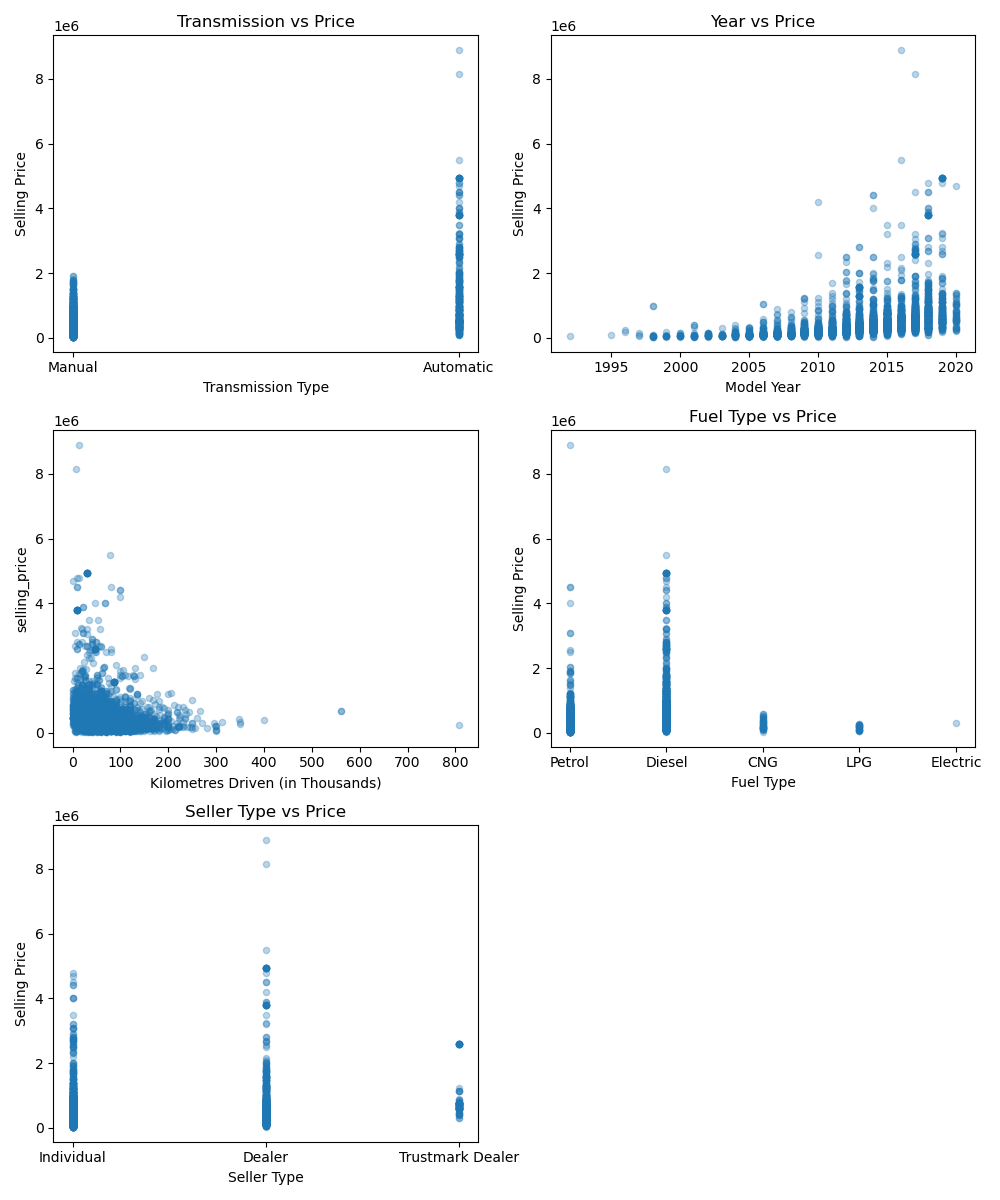
\includegraphics[width=0.95\textwidth]{../figures/car_price_vs_variables.png}
  \caption{Selling price versus key vehicle characteristics such as year, mileage, fuel type, transmission, and seller type.}
\end{figure}

The visual analysis also shows that fuel type, transmission, seller type, and owner history influence the observed price to a lesser extent. Some categories appear associated with price premium, although their influence is less direct than the effect of model year and kilometres driven.

\section{Correlation Analysis}
A correlation analysis was used to examine the linear associations between the numerical predictors and the target variable. The overall structure indicates that the year of manufacture and kilometres driven are among the most important numerical drivers of price. The categorical variables were also examined through encoded representations to assess their contribution to the modelling task.

\begin{figure}[H]
  \centering
  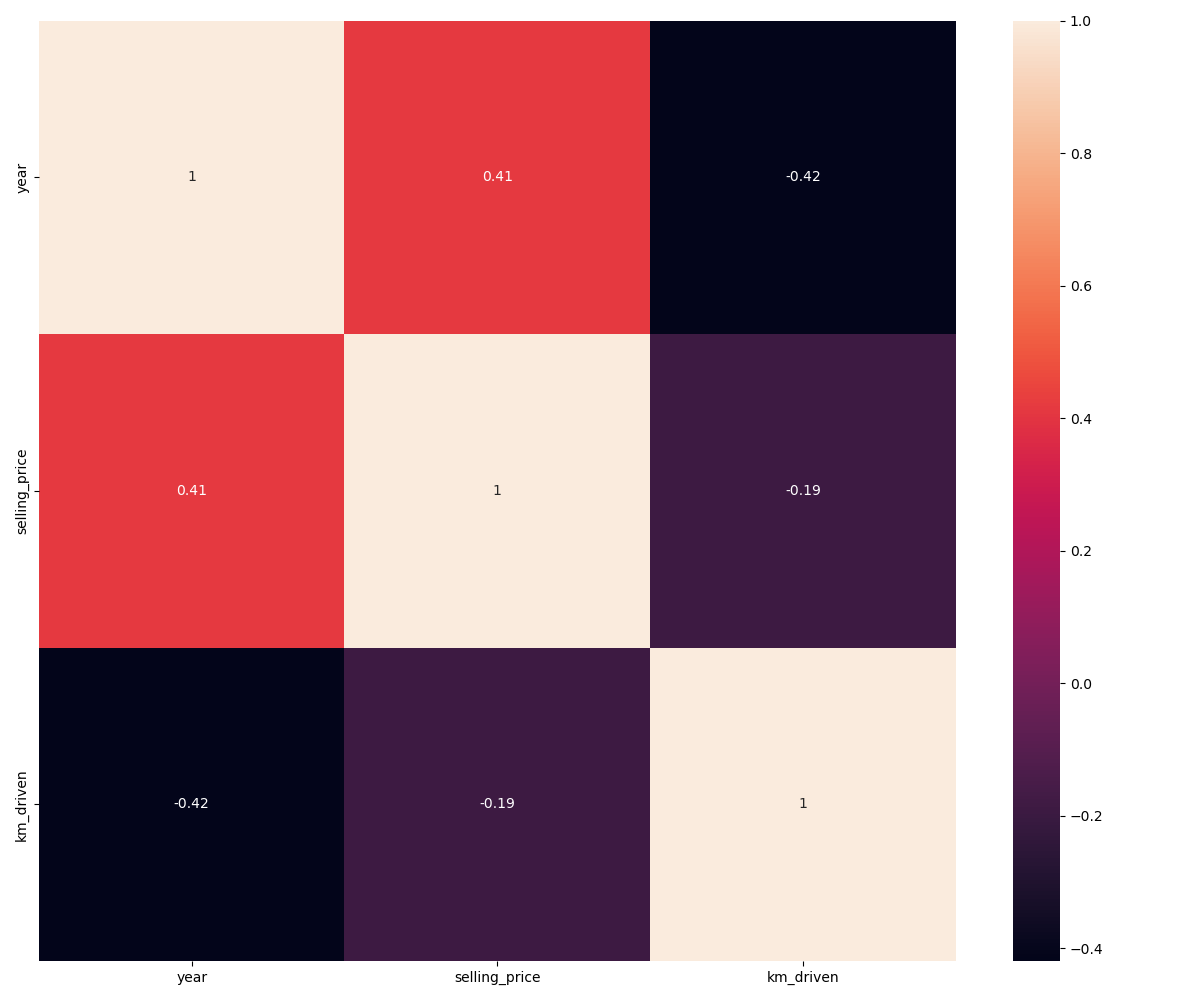
\includegraphics[width=0.95\textwidth]{../figures/variable_correlations.png}
  \caption{Correlation structure among the encoded numerical features and the target variable.}
\end{figure}

\begin{figure}[H]
  \centering
  
\includegraphics[width=0.95\textwidth]{../figures/condensed_variable_correlations.png}
  \caption{Condensed view of the association structure across the mixed categorical and numerical features.}
\end{figure}

\chapter{Model Development and Evaluation}
\section{Regression Models Compared}
Several regression models were trained and compared to identify the most suitable approach for this prediction task. The analysis focused on baseline linear regression and regularized regression methods, including Ridge and Elastic Net, which are useful for handling multicollinearity and high-dimensional encoded features.

The evaluation was based on two standard metrics:
\begin{itemize}
  \item Root Mean Squared Error (RMSE), which penalizes larger errors more strongly; and
  \item the coefficient of determination, $R^2$, which measures how much of the variation in selling price is captured by the model.
\end{itemize}

\begin{table}[H]
  \centering
  \caption{Performance comparison of the evaluated regression models.}
  \begin{tabular}{lcc}
    \toprule
    Model & RMSE & $R^2$ \\
    \midrule
    Linear Regression (train-test split) & 395243.69 & 0.49 \\
    Ridge Regression (alpha $=1.0$) & 358161.94 & 0.58 \\
    Elastic Net (cross-validation summary) & 286774.45 & 0.74 \\
    \bottomrule
  \end{tabular}
\end{table}

These results indicate that regularized models improve the predictive performance compared with the simple linear baseline. The Elastic Net model, in particular, achieved the strongest average cross-validated performance, suggesting that penalized linear regression is a useful starting point for this dataset.

\section{Model Interpretation}
The results suggest that changes in price are strongly related to vehicle age and usage. The year of manufacture and kilometres driven are the most meaningful signals in the data, while categorical variables such as fuel type, transmission, and seller type introduce additional structure that the regression model can exploit. The improvements observed with regularized models show that the encoded feature space benefits from shrinkage and that simple linear assumptions can still capture a considerable portion of the price variation.

\chapter{Discussion}
This project demonstrates that used car prices can be predicted reasonably well using a small set of interpretable features. The strongest patterns are those associated with depreciation: newer cars and cars with lower mileage are generally more expensive. The inclusion of categorical information also added useful predictive power, especially when combined with regularization.

The main limitation of the present approach is that the relationship between price and vehicle attributes is likely not purely linear. Some categories and combinations of features may interact in ways that are not fully captured by linear regression alone. Nevertheless, the results show that the baseline regression models provide a solid foundation and are appropriate for a first analytical study.

Future work could extend this project by testing more flexible models such as decision trees, random forests, gradient boosting, and other nonlinear regressors. Feature engineering around vehicle make and model, condition, and market trends could further improve predictive accuracy.

\chapter{Conclusion}
This project successfully developed and evaluated a regression workflow for used car price prediction. The analysis showed that vehicle age, mileage, and a small set of categorical attributes contain enough information to estimate resale prices with moderate accuracy. Among the models tested, regularized linear regression methods delivered the best overall results and outperformed the simple linear baseline.

Overall, the study confirms that regression-based methods are a suitable starting point for used car price prediction and that linear models can provide both good predictive performance and interpretability for this type of problem.
